
\section{Method}\label{sec:methods}
For this review, we followed the guidelines proposed by \citet{kitchenham2009systematic} and framed the search using the PICOC criteria \citep{petticrew2008systematic}:
\begin{itemize}
    \item \textbf{Population}: Applications, Developers
    \item \textbf{Intervention}: Collaborative, multi-user and interactive \gls{AR} applications
    \item \textbf{Comparison}: Students' results in classes using AR applications with classes that do not
    \item \textbf{Outcome}: Effectiveness in increasing understanding of a topic
    \item \textbf{Context}: Education, primary or secondary schools
\end{itemize}

Once the research questions have been defined, the literature review is split into three steps: planning, conducting and reporting. We used the online tool Parsifal\footnote{parsif.al} to conduct the first two steps of the review while the third was performed using Google Forms and collecting the results in a spreadsheet. The results of the data collection, as well as the code used to generate the figures in this document, is available on Github\footnote{\textless removed for review\textgreater}
%github.com/Stocastico/AR\_SLR\_Paper}.

\subsection{Study selection}
The aim of this phase is to select the papers which are relevant for the systematic review, define the inclusion and exclusion criteria, and to provide the categories for the analysis.
We have selected four digital libraries as source: IEEExplore, Scopus, Springer and ISI Web of Science. We used the search terms \emph{Augmented Reality}, \emph{Education} $\lor$ \emph{Learning}, \emph{Collaborative} $\lor$ \emph{Interactive} $\lor$ \emph{Multi-user}, \emph{Application} $\lor$ \emph{Evaluation}. For this work, we did not consider papers which appeared online after the first of October 2020. The search returned \allPapers results, of which \duplPapers were marked as duplicates. We read the abstract of the remaining \papersCheckAbstract articles and, applying the inclusion and exclusion criteria specified below, we were left with \papersToRead articles. We finally proceeded to read the selected articles and excluded \papersExludedAfterReading further articles, thus selecting \papersSelected articles for the literature review.
Table \ref{tab:searchstring} summarises the selection process, specifying the search string used for each digital library as well as the number of papers returned, marked as duplicated and selected for the systematic review.

As inclusion criteria, we required the studies to be published in 2015 or afterwards and that they describe an AR app which has actually been implemented. The exclusion criteria are the following:

\begin{itemize}
    \item The application described is not interactive, multi-user or collaborative
    \item The paper does not describe an AR application
    \item The paper describes an unrelated application (e.g. for museums or clinical training)
    \item The target audience is outside the specified age range (5 - 18 years old students)
    \item The paper is not peer reviewed
    \item The paper is not written in English
\end{itemize}

Fig. \ref{fig:flowchart} shows a flowchart depicting the systematic review process. The \papersToRead papers were reviewed by three researchers. To compute the interrater agreement, two researchers read a set of 50 abstracts randomly selected from all the studies (excluding duplicates) and 10 papers (among the \papersSelected selected paper). The interrater agreement, as defined in \citep{cohen1960coefficient} was $0.88$ for the abstracts and $0.73$ for the papers.

% \begin{figure}[ht]	
% 	\begin{center}
% 	%\includesvg[width=0.48\textwidth]{figures/prisma}
% 	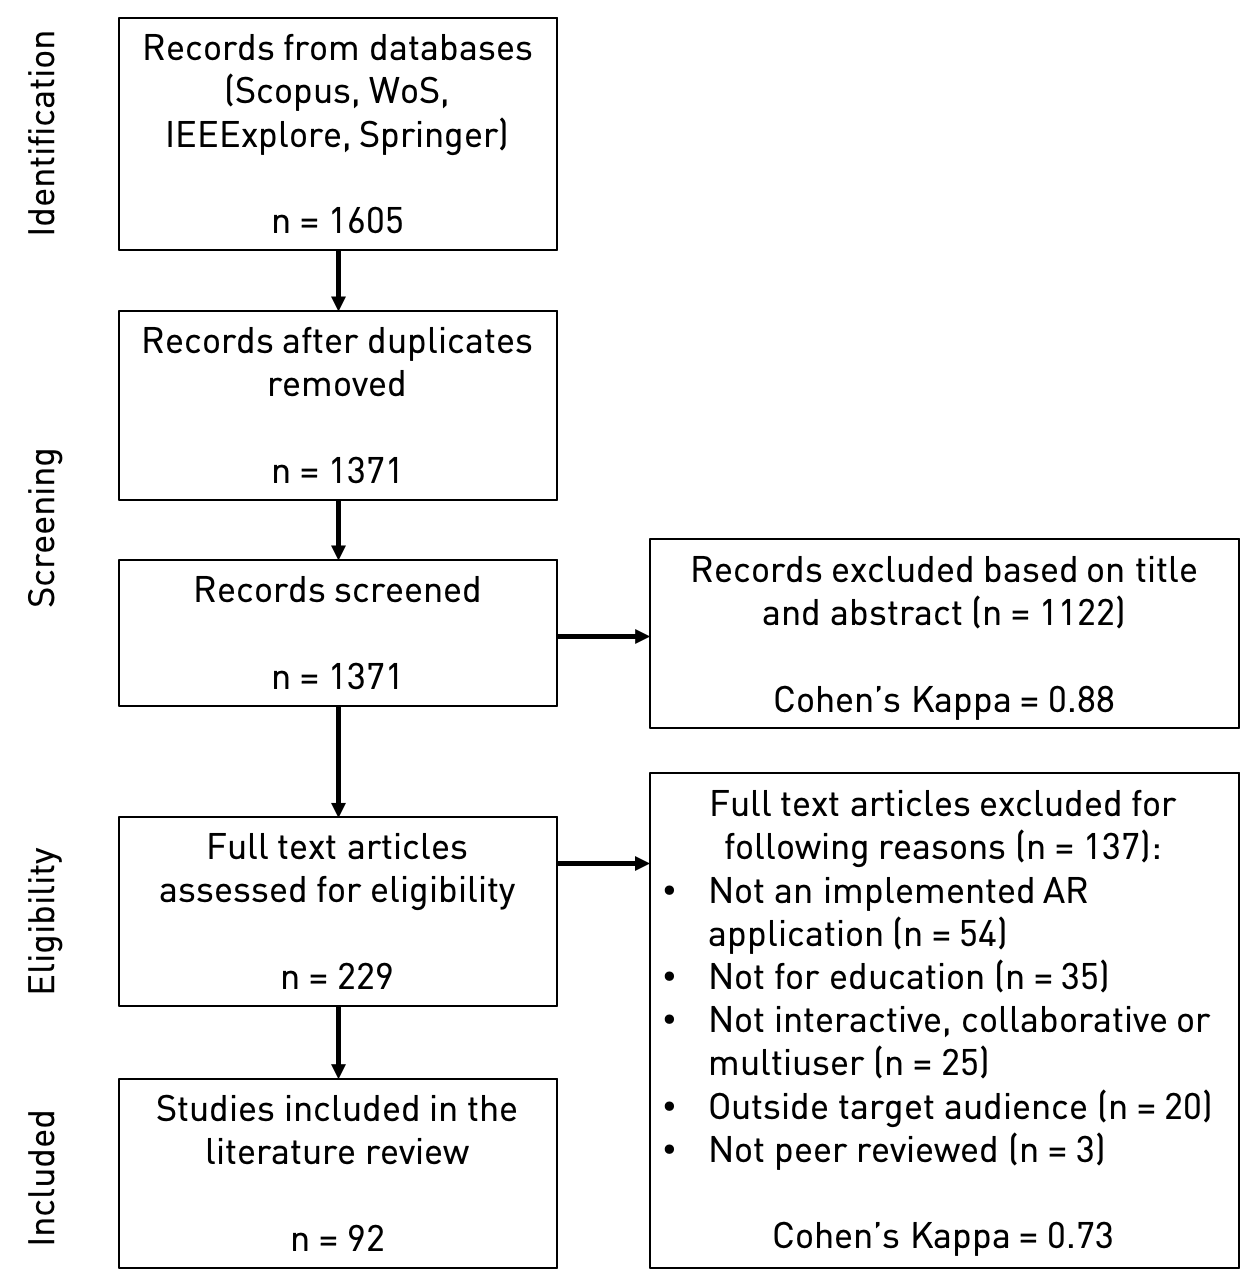
\includegraphics[width=0.6\textwidth]{figures/prisma.png}
% 	\caption{Prisma flowchart of the search protocol.}
% 	\label{fig:flowchart}
%     \end{center}
% \end{figure}


% \begin{table*}[htbp]
% \small
% \centering
% \caption {Query strings and number of papers returned.}\label{tab:searchstring}
% \begin{tabular}{|M{1.9cm}||M{8cm}|M{1.25cm}|M{1.85cm}|M{1.45cm}|}
%     \hline
%          \textbf{Digital Library} & \textbf{Query string} & \textbf{Papers} & \textbf{Duplicates} & \textbf{Selected} \\
%     \hline
%     \hline
%          IEEExplore    &  (``All Metadata'': ``Augmented reality'' AND (``Education'' OR ``Learning'') AND (``Collaborative'' OR ``Interactive'' OR ``multi-user'' OR ``multi-user'') AND (``Application'' OR ``Evaluation'')) Filters Applied: 2015 - 2020 & 116 & 47 & \textbf{32} \\
%     \hline
%         Scopus         & TITLE-ABS-KEY ( ``Augmented reality''  AND  ( ``Education''  OR  ``Learning'' )  AND  ( ``Interactive''  OR  ``multi-user''  OR  ``multiuser'' )  AND  ( ``Application''  OR  ``Evaluation'' ) )  AND  ( PUBYEAR $>$ 2014 )  & 476 & 65 & \textbf{92} \\
%     \hline
%         Springer       & (collaborative OR interactive OR multiuser OR multi-user) AND ``augmented reality'' AND (education OR learning) AND (primary OR secondary) AND (application OR evaluation)
% within Chapter - Conference Paper  2015 - 2020  & 803 & 67 & \textbf{58} \\
%     \hline
%         Web of Science & ``Augmented reality'' AND (``Education'' OR ``Learning'') AND (``Collaborative'' OR ``Interactive'' OR ``multi-user'' OR ``multiuser'') AND (``Application'' OR ``Evaluation'') & 210 & 55 & \textbf{47} \\
%     \hline

% \end{tabular}
% \end{table*}